\section{Videojuego}
En este apartado se dará la definición de un videojuego y aquello que involucra, la clasificación que existe para ellos, como se encuentra en la actualidad la industrial mundial del videojuego, luego de manera específica un pequeño estudio de mercado en México con solo los campos que nos interesan para el proyecto y finalmente el desarrollo que existe de los videojuegos dentro de la industria en México. 

\subsection{Definición}
Un videojuego es un medio de entretenimiento que involucra a un usuario, denominado jugador, en una interacción constante entre una interfaz y un dispositivo de video según Morales Urrutia\cite{defVid}. Los videojuegos recrean	entornos y situaciones virtuales en los que el jugador puede controlar la situación para alcanzar objetivos por medio de determinadas reglas. La interacción se lleva a cabo mediante dispositivos de salida y de entrada.
\\[1pt]
		
Los videojuegos arte, ciencia y tecnología; involucran una gran cantidad de habilidades y conocimientos en distintas disciplinas, desde ciencias formales hasta ciencias sociales que van más allá del típico proyecto de software e implican al mismo tiempo la creatividad y la imaginación.
\\[1pt]

Su propósito de igual manera es muy variado, puede ser con fines solo de entretenimiento, aprendizaje, simulación, terapia física o emocial, y más. El propósito de un videojuego puede ser siempre definido, pero tambien puede tener como consecuencia otros resultados benéficos o no.
\\[1pt]

Ya que los propósitos de un videojuego dependen del enfoque que se le quiera dar, nos tenemos que apoyar a quien va dirigido nuestro contenido. Un videojuego puede ir dirigido a cualquier persona, esto determinará después los elementos u objetivos que se quieren conseguir.
\\[1pt]  
					
\subsection{Clasificación}
La clasificación es un proceso que permite una ordenación de elementos, según determinados criterios. Así se reunen en grupos que comparten características similares con fines de organización y facilitar la comunicación respecto de un tema. Primero hablaremos de las clasificaciones que se estan discutiendo para los videojuegos y después según las necesidades del proyecto tomaremos las convenientes. 
\\[1pt]

El documento MDA\cite{vid10} (por sus siglas en inglés) establece los tres aspectos fundamentales, Mecánicas, Dinámicas y Estética como un marco de referencia para entender los juegos y hacer una mejor clasificación de ellos. Las mecánicas, son las reglas y sistemas que crean nuestra experiencia de juego, sus componentes particulares a nivel representación de datos y algoritmos; las dinámicas, describen el comportamiento de las mecánicas en respuesta a las acciones del jugador; y la estética, define la respuesta emocional evocada por el usuario cuando interactúa con el juego. Aunque esta clasificación abarca a todos los videojuegos existentes, no son considerados comúnmente en la industria, por esa razón no se tomará dicha clasificación.
\\[1pt]

Mark Wolf\cite{vid11} enfatiza la diferencia fundamental de los videojuegos con otros medios y el por qué de ser necesaria una categorización en géneros muy distinta a la aplicable a libros y películas. Pues la participación del jugador es el determinante a la hora de describir y clasificar juegos de video. Mark Wolk comenta que "Por supuesto, cualquier sistema propuesto será objeto de debate y crítica. Al mismo tiempo, aparecer con un listado consistente y comprensivo que intenta definir y articular las fronteras de cada uno, es una tarea mucho más difícil que criticar otros ya existentes". Donde se vuelve a comentar el problema de la no existencia de una clasificación determinada para los videojuegos.
\\[1pt]

Así que, se abarcarán dos de las clasificaciones determinadas por el mercado de la industria. La clasificación por contenido, que son definidas por asuntos legales que competen a cada región y la clasificación por géneros que son las razones emotivas o de experiencia que tenemos dentro del videojuego.
\\[1pt]

\subsubsection{Clasificación por contenido}

	Es usado para el control y supervisión de contenido y asi determinar el público al cual puede ser mostrado.  Existen diferentes sistemas en el mundo donde la mayoría de estos están asociados y patrocinados por un gobierno y a veces forman parte del sistema de clasificación de películas del país.Existen hasta el momento diecinueve tipos diferentes de clasificación por contenido.\\[1pt]	
	
	México pertenece a la Junta de Clasificación de Software de Entretenimiento (ESRB, Entertainment Software Rating Board)\cite{vid02}. La pertenencia a esta clasificación se debe a la cercanía con EUA que tiene el país y el constante comercio que comparten. Esta clasificación proporciona una información concisa y objetiva acerca del contenido de los juegos de video y las aplicaciones para que los consumidores, en especial los padres, puedan tomar decisiones informadas. La clasificación de la ESRB constan de tres partes; edad, descriptor de contenido y elementos interactivos.\\[1pt]
			
\textbf{Por edad}
\\[1pt]
En donde se sugieren la edad adecuada para el juego. La imagen \ref{fig:clasEti} muestra la simbología usada por edad. Esta representación es usada tal cuál en los empaques del videojuego. A continuación se enlistan los apartados por edad que existen y a que público pertenecen.	
\\[1pt]

	\begin{figure}
	\centering 
	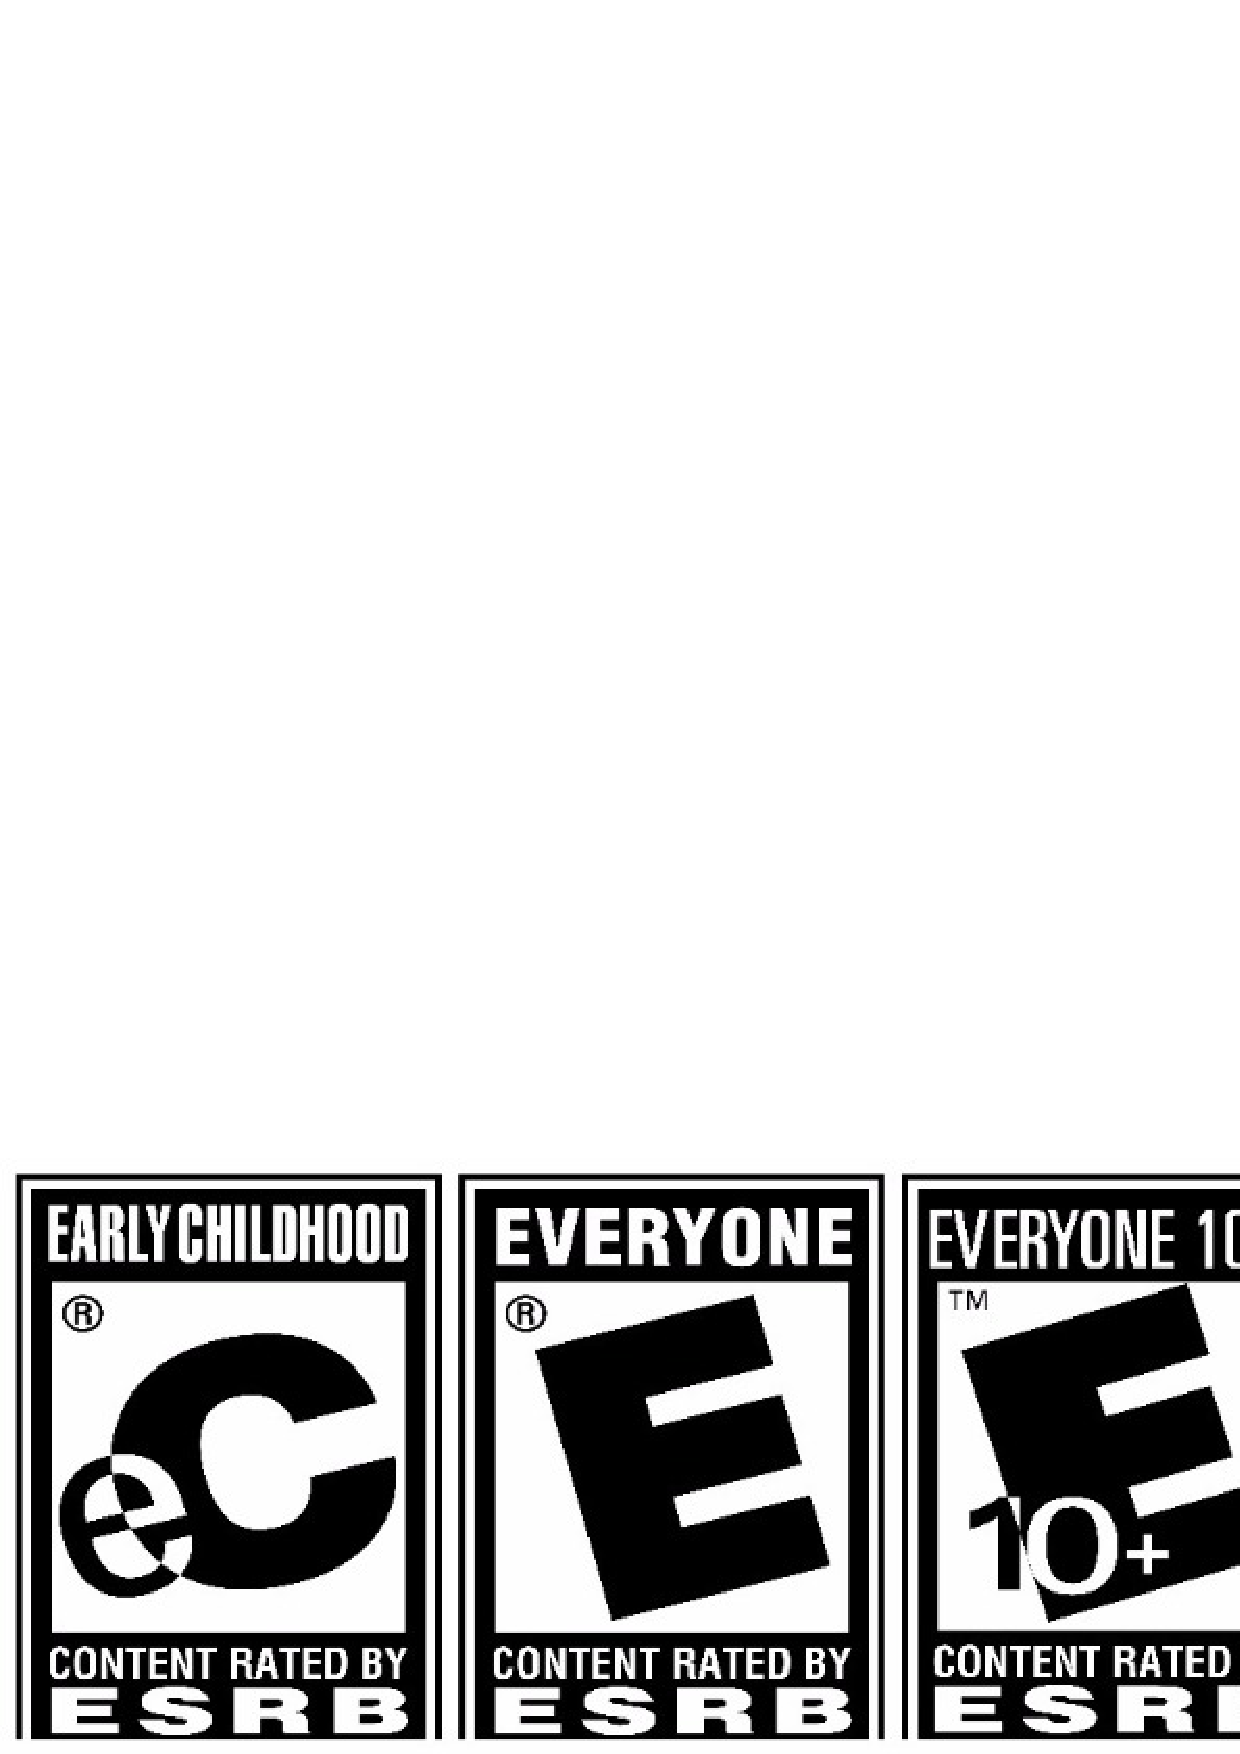
\includegraphics[width=\textwidth]{03MarcoTeorico/imageR/clasEti}
	\caption{Etiquetas de clasificación por edad en un videojuego.}
	\label{fig:clasEti}
\end{figure}


			\begin{itemize}
			\item Niños pequeños: 
			El contenido está dirigido a niños pequeños menores de diez años.
			
			\item Todos: 
			El contenido por lo general es apto para todas las edades. Puede que contenga una cantidad mínima de violencia de caricatura, de fantasía o ligera, o uso poco frecuente de lenguaje moderado.
			
			\item Todos +10: 
			El contenido por lo general es apto para personas de diez años o más. Puede que contenga más violencia de caricatura, de fantasía o ligera, lenguaje moderado o temas mínimamente provocativos.
			
			\item Adolescentes: 
			El contenido por lo general es apto para personas de trece años o más. Puede que contenga violencia, temas insinuantes, humor grosero, mínima cantidad de sangre, apuestas simuladas o uso poco frecuente de lenguaje fuerte.
			
			\item Maduro: 
			El contenido por lo general es apto para personas de diecisiete años o más. Puede que contenga violencia intensa, derramamiento de sangre, contenido sexual o lenguaje fuerte.
			
			\item Adultos únicamente: 
			El contenido es apto sólo para adultos de dieciocho años o más. Puede que incluya escenas prolongadas de violencia intensa, contenido sexual gráfico o apuestas con moneda real.
			
			\item Clasificación pendiente: 
			Aparece solo en material de publicidad, de comercialización y promocional en relación con un videojuego "en caja" que se espera que lleve una clasificación de la ESRB y debe reemplazarse por la clasificación del juego una vez que haya sido asignada.
			
		\end{itemize}		
			
			\textbf{Descriptores de contenido: } 
			\\[1pt]
			Indican los elementos que pueden haber motivado la clasificación asignada y pueden resultar de interés o preocupación para el comprador. La imagen \ref{fig:clasDes} muestra una etiqueta con los descriptores en una etiqueta a lado de la edad sugerida. A continuación se enlistan los descriptores de contenido que existen al momento y en breve una explicación. 
			\\[1pt]
				\begin{figure}
				\centering
				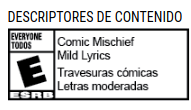
\includegraphics[width=0.3\textwidth]{03MarcoTeorico/imageR/clasDes}
				\caption{Muestra de descriptor de contenido de un videojuego.}
				\label{fig:clasDes}
			\end{figure}
			
			
			\begin{itemize}
				\item Referencia al alcohol: Referencia e imágenes de bebidas alcohólicas.
				\item Animación de sangre: Representaciones decoloradas o no realistas de sangre.
				\item Sangre: Representaciones de sangre.
				\item Derramamiento de sangre: Representaciones de sangre o mutilación de partes del cuerpo.
				\item Violencia de caricatura: Acciones violentas que incluyen situaciones y personajes caricaturescos. Puede incluir violencia en la cual un personaje sale ileso después de que la acción se llevó a cabo.
				\item Travesuras cómicas: Representaciones o diálogo que impliquen payasadas o humor sugestivo.
				\item Humor vulgar: Representaciones o diálogo que implique bromas vulgares.
				\item Referencia a drogas: Referencia o imágenes de drogas.
				\item Violencia de fantasía: Acciones violentas de naturaleza fantástica que incluyen personajes humanos y no humanos en situaciones que se distinguen con facilidad de la vida real.
				\item Violencia intensa: Representaciones gráficas y de apariencia realista de conflictos físicos. Puede comprender sangre excesiva o realista, derramamiento de sangre, armas y representaciones de lesiones humanas y muerte.
				\item Lenguaje: Uso de lenguaje inadecuado de moderado a intermedio.
				\item Letra de canciones: Referencias moderadas de lenguaje inadecuado, sexualidad, violencia, alcohol o uso de drogas en la música.
				\item Humor para adultos: Representaciones o diálogo que contienen humor para adultos, incluidas las alusiones sexuales.
				Desnudez: Representaciones gráficas o prolongadas de desnudez.
				\item Desnudez parcial: Representaciones breves o moderadas de desnudez.
				\item Apuestas reales: El jugador puede apostar, incluso colocar apuestas con dinero o divisas de verdad.
				\item Contenido sexual: Representaciones no explícitas de comportamiento sexual, tal vez con desnudez parcial.
				\item Temas sexuales: Alusiones al sexo o a la sexualidad.
				\item Violencia sexual: Representaciones de violaciones o de otros actos sexuales violentos.
				\item Apuestas simuladas: El jugador puede apostar sin colocar apuestas con dinero o divisas reales.
				\item Lenguaje fuerte: Uso explícito o frecuente de lenguaje soez.
				Letra de canciones fuerte: Alusiones explícitas o frecuentes de lenguaje inadecuado, sexo, violencia o uso de alcohol o drogas en la música.
				\item Contenido sexual fuerte: Alusiones explícitas o frecuentes de comportamiento sexual, tal vez con desnudez.
				\item Temas insinuantes: Referencias o materiales provocativos moderados.
				\item Referencia al tabaco: Referencia o imágenes de productos de tabaco.
				\item Uso de alcohol: Consumo de alcohol o bebidas alcohólicas.
				\item Uso de drogas: Consumo o uso de drogas.
				\item Uso de tabaco: Consumo o uso de productos de tabaco.
				\item Violencia: Escenas que comprenden un conflicto agresivo. Pueden contener desmembramiento sin sangre.
				Referencias violentas: Alusiones a actos violentos.
			\end{itemize}
			
			\textbf{Elementos interactivos: } 
			\\[1pt]
			Informan acerca de los aspectos interactivos de los productos, incluida la capacidad de los usuarios de interactuar, o si se comparte la ubicación de los usuarios con otros usuarios. La imagen \ref{fig:clasInt} da como ejemplo en una caja de videojuegos como se vería. 
			\\[1pt]
			
				\begin{figure}
				\centering
				
\includegraphics[width=0.5\textwidth]{03MarcoTeorico/imageR/clasInt}
				\caption{Ejemplo de como se muestra los elementos interactivos en el empaque de un videojuego.}
				\label{fig:clasInt}
				\end{figure}
			
			
			\begin{itemize}
			
			\item Ubicación compartida: Incluye la capacidad de mostrar la ubicación del usuario a otros usuarios de la aplicación.
			\item Interacción de usuarios: Indica una posible exposición a contenido sin filtro y sin censura generado por usuarios, que incluye comunicaciones y medios compartidos de usuario a usuario a través de medios y redes sociales.
			\item Compras digitales: Permite la compra de productos digitales directamente desde la aplicación.
			\item Internet sin límites: El producto brinda acceso a Internet.
		\end{itemize}
		
	\subsubsection{Clasificación por género}
 La clasificación por géneros se conforman en torno a factores como: la representación gráfica, el tipo de interacción entre el jugador y la máquina, la ambientación, y su sistema de juego, siendo este último el criterio más habitual a tener en cuenta. A lo largo de la historia de los videojuegos, sus creadores han ido dando lugar a una variedad creciente de géneros en las distintas plataformas disponibles y muchas de la veces son combinables entre sí. Por lo dicho anteriormente de la clasificación, existen diferentes divisiones y subdivisiones por varios autores. A continuación se presenta una de ellas en la imagen \ref{fig:vidGen} por Luis Chong y que a nuestra consideración se tomará.
	\\[1pt]
	
	\begin{figure}
		\centering
		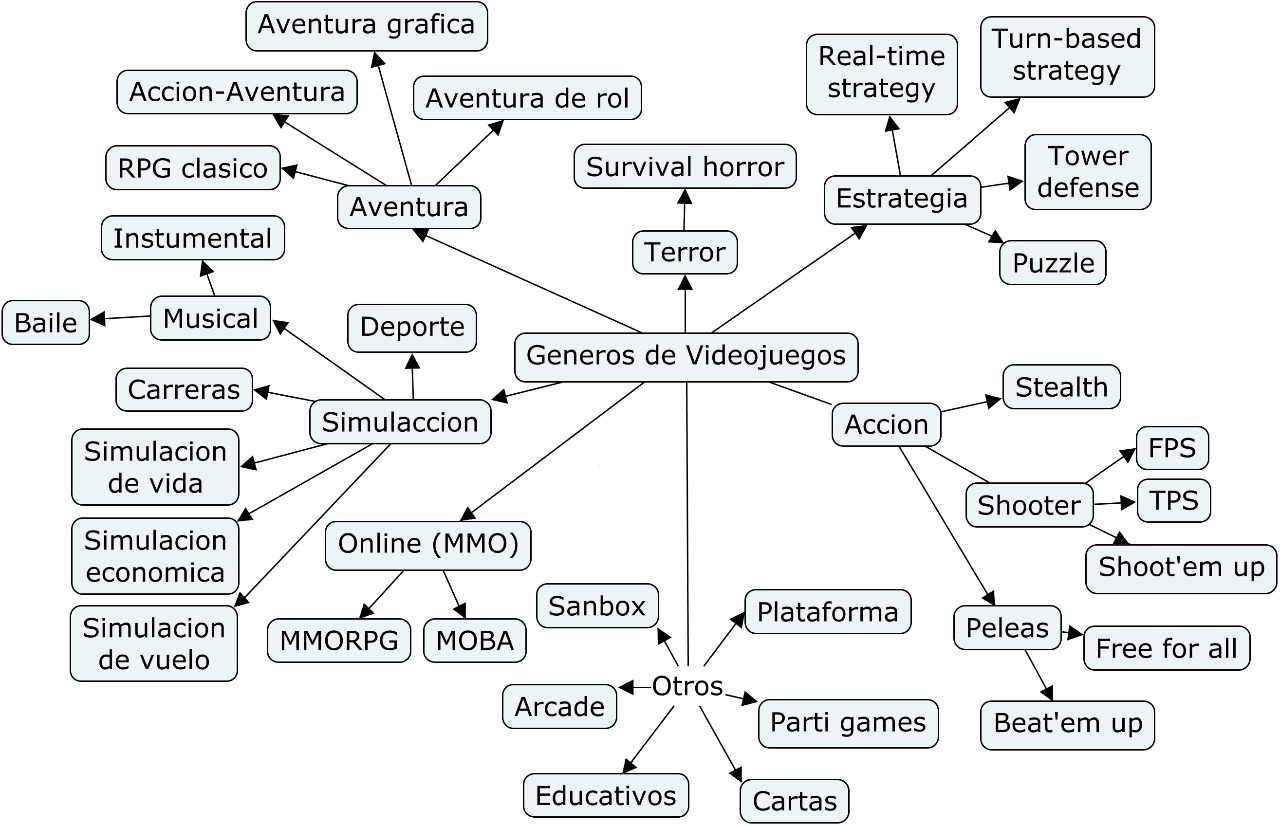
\includegraphics[width=\textwidth]{03MarcoTeorico/imageR/gene}
		\caption{Géneros de videojuegos propuesto por Luis Chong[Imagen](2015). Recuperado de: https://www.emaze.com/@AFRICWZL/Tesis-Artes-Digitales.}
		\label{fig:vidGen}
	\end{figure}	
	
		
\subsection{Industria mundial}
			 
			 La industria mundial refleja el nivel de consumo que existe. El videojuego surge en 1952; no obstante, el videojuego como industria surgiría hasta 1972, logrando su mayor revolución durante la década de los 80`s. 
			 \\[1pt]
			 
			 Según un estudio elaborado por la empresa Newzoo en la imagen \ref{fig:newzooIndMun}, la industria del videojuego generará 108.900 millones de dólares de ingresos totales, de los que se espera que hasta 94.400 millones corresponden solamente a ventas digitales, que representa un 87\% del mercado mundial. Actualmente la industria del videojuego, también llamada industria del ocio virtual, es la industria del entretenimiento, superando a la industria del cine y la música. Ya que hemos visto el consumo de videojuegos ahora nos vamos a su plataforma que nos interesa, que son los dispositivos móviles.
			 \\[1pt]	
			 
			 El segmento de los dispositivos móviles (Smartphones y tablets) es el que aporta más dinero en la industria del videojuego. Este sector copa un 42\% del mercado y su consumo ha tenido un crecimiento del 19\% con respecto al año anterior. Se espera que generen un ingreso de 46.100 millones de dólares. A día de hoy no se entiende a ninguna persona sin su Smartphone en la mano y esto hace que un gran porcentaje de usuarios juegue a algún tipo de juego en su teléfono y hasta utilice navegadores de internet sin necesidad de instalar nada. Se espera que en 2020 acaparen el 50\% del mercado. \cite{vid01}
			 \\[1pt]   
			 
			 	\begin{figure}
			 	\centering
			 	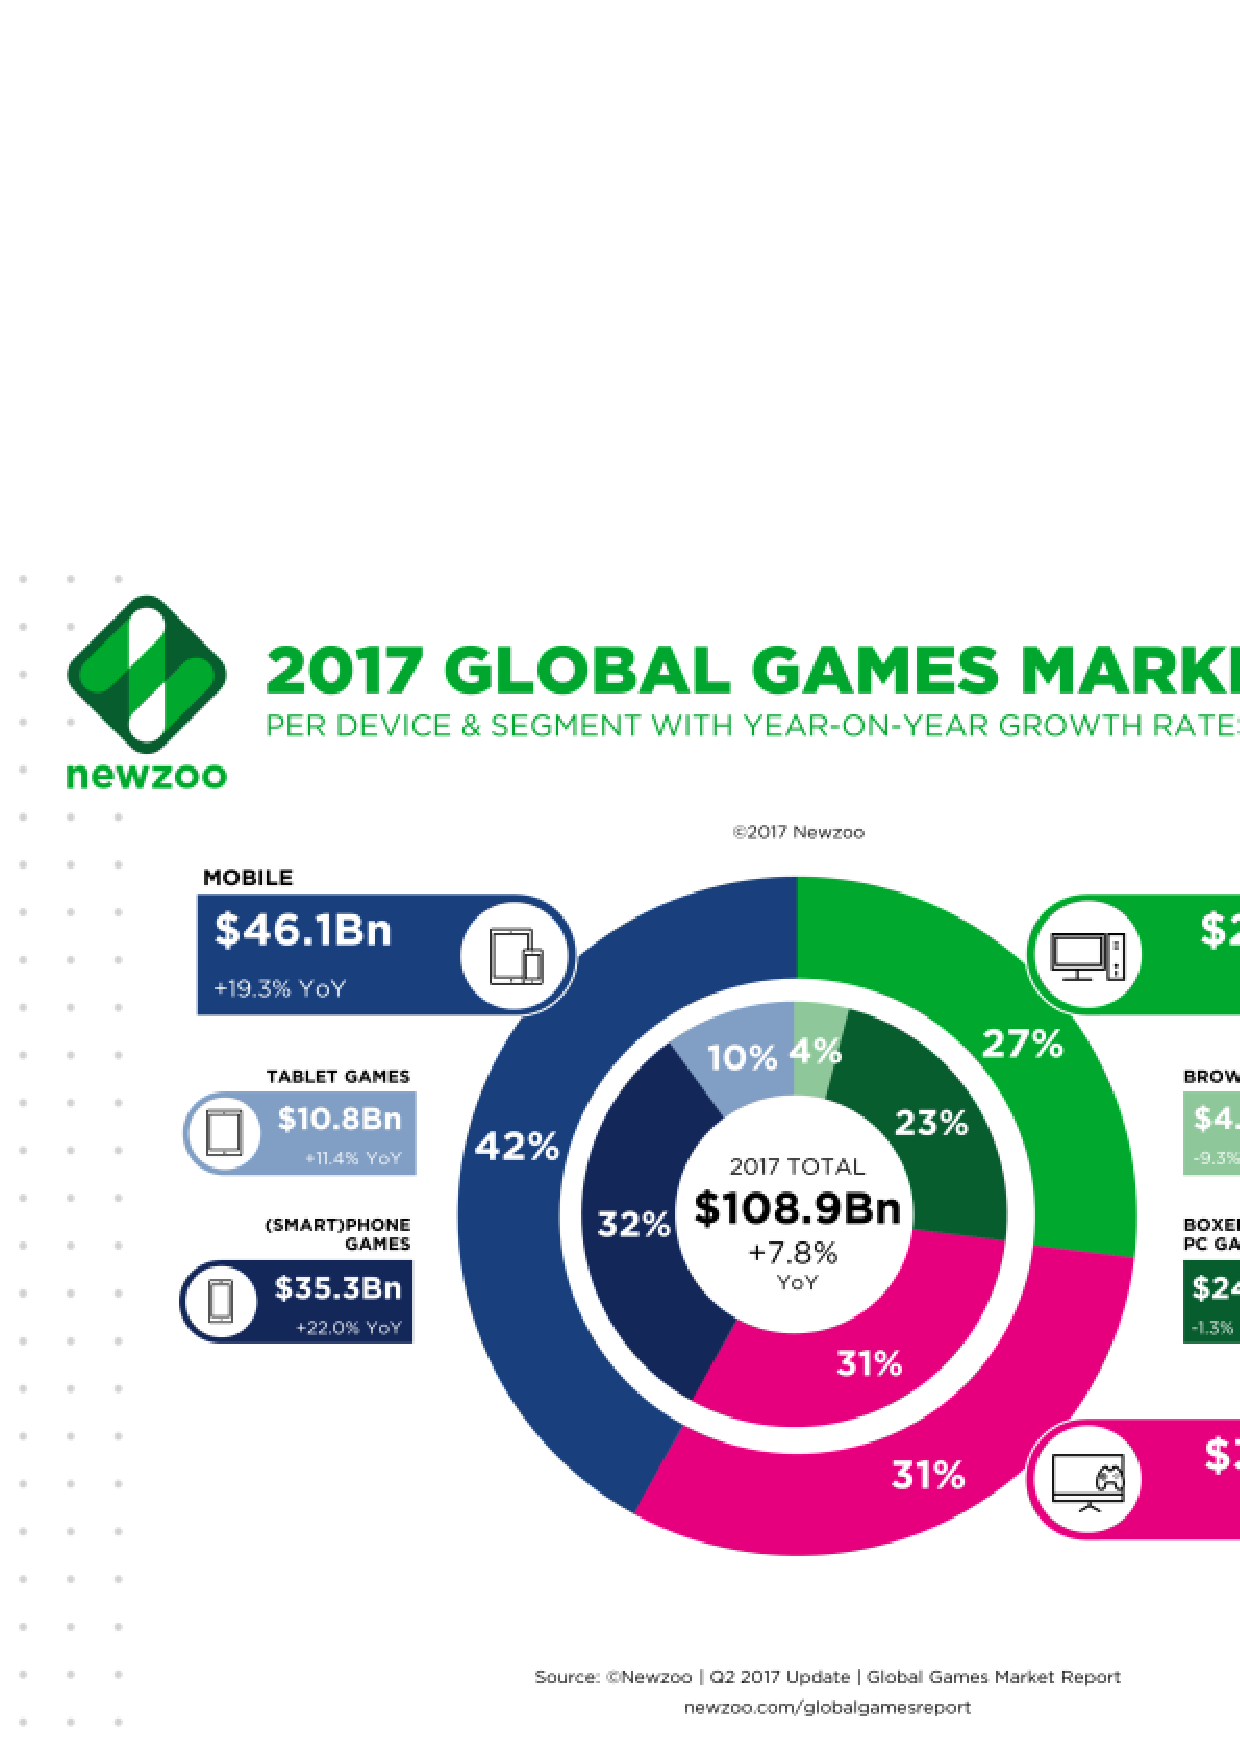
\includegraphics[width=\textwidth]{03MarcoTeorico/imageR/newzooIndMun}
			 	\caption{Mercado global de juegos por dispositivo y segmento con tasas de crecimiento interanual al año 2017.[Imagen](2017). Recuperado de: https://newzoo.com/resources/}
			 	\label{fig:newzooIndMun}
			 \end{figure}	
		 
		 Sabiendo lo anterior podemos ver la conveniencia que existe de realizar un videojuego dentro de los dispositivos móviles.
			 
			 
\subsection{Estudio de mercado en México}

Históricamente, México ha sido el país numero uno en el consumo de videojuegos en Latinoamérica como se ve en la imagen \ref{fig:mexicoUno}. Esto se debe a su cercanía con los Estados Unidos. Esto genera que se de una transmisión cultural y de tecnología casi inmediata. La industria de los videojuegos en México es cosa seria. 
\\[1pt] 
	\begin{figure}
	\centering
	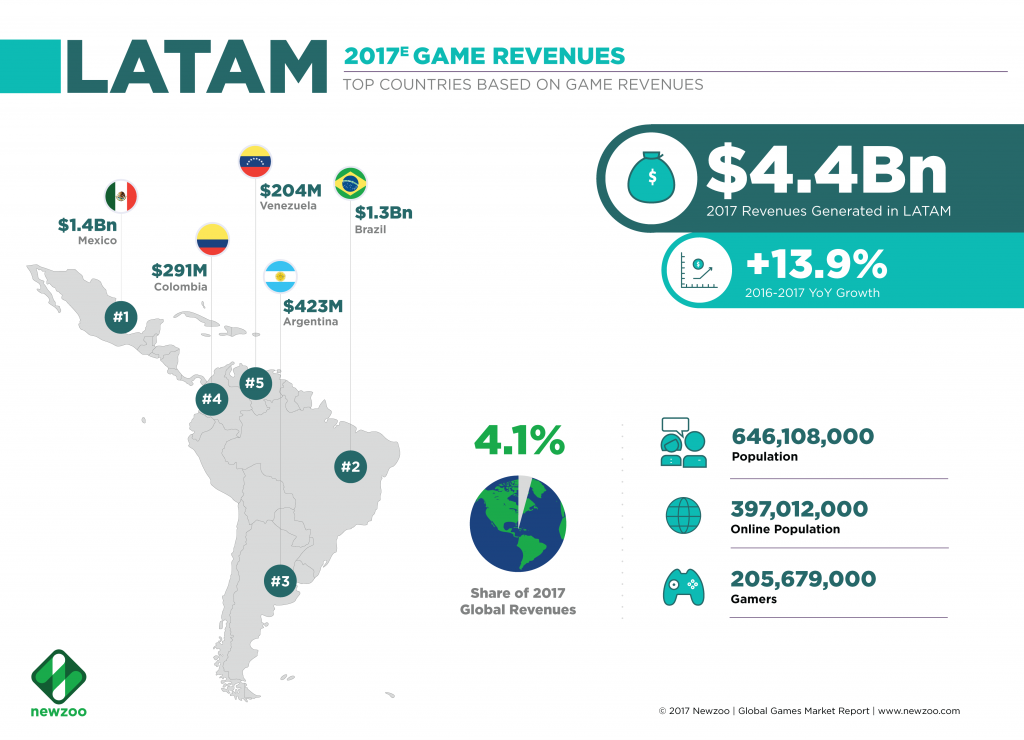
\includegraphics[width=\textwidth]{03MarcoTeorico/imageR/mexicoUno}
	\caption{Ingresos del juego en latinoamérica al año 2017.[Imagen](2017). Recuperado de: https://newzoo.com/resources/}
	\label{fig:mexicoUno}
	\end{figure}

Mientras que la economía nacional este mercado de entretenimiento pronostica un crecimiento anual de 8.4\% para 2017, es decir, casi cuatro veces lo que creció el Producto Interno Bruto (PIB) hace un año y lo que avanzaría al cierre del periodo en curso. De acuerdo con el estudio “Jugar no es cosa de niños: Dimensionamiento del Mercado de Videojuegos en México 1Q17” como se muestra en la imagen \ref{merVidMex}, elaborado por The Competitive Intelligence Unit (The CIU), este mercado tuvo ingresos por más de 22,852 millones pesos (mdp) en 2016, esto es, 13.3\% más con respecto al año anterior, con un número de usuarios de más de 65 millones \cite{vid03}. Y como lo analizamos en la industria mundial, también veremos los videojuegos en los dispositivos móviles.
\\[1pt] 
\begin{figure}
	\centering
	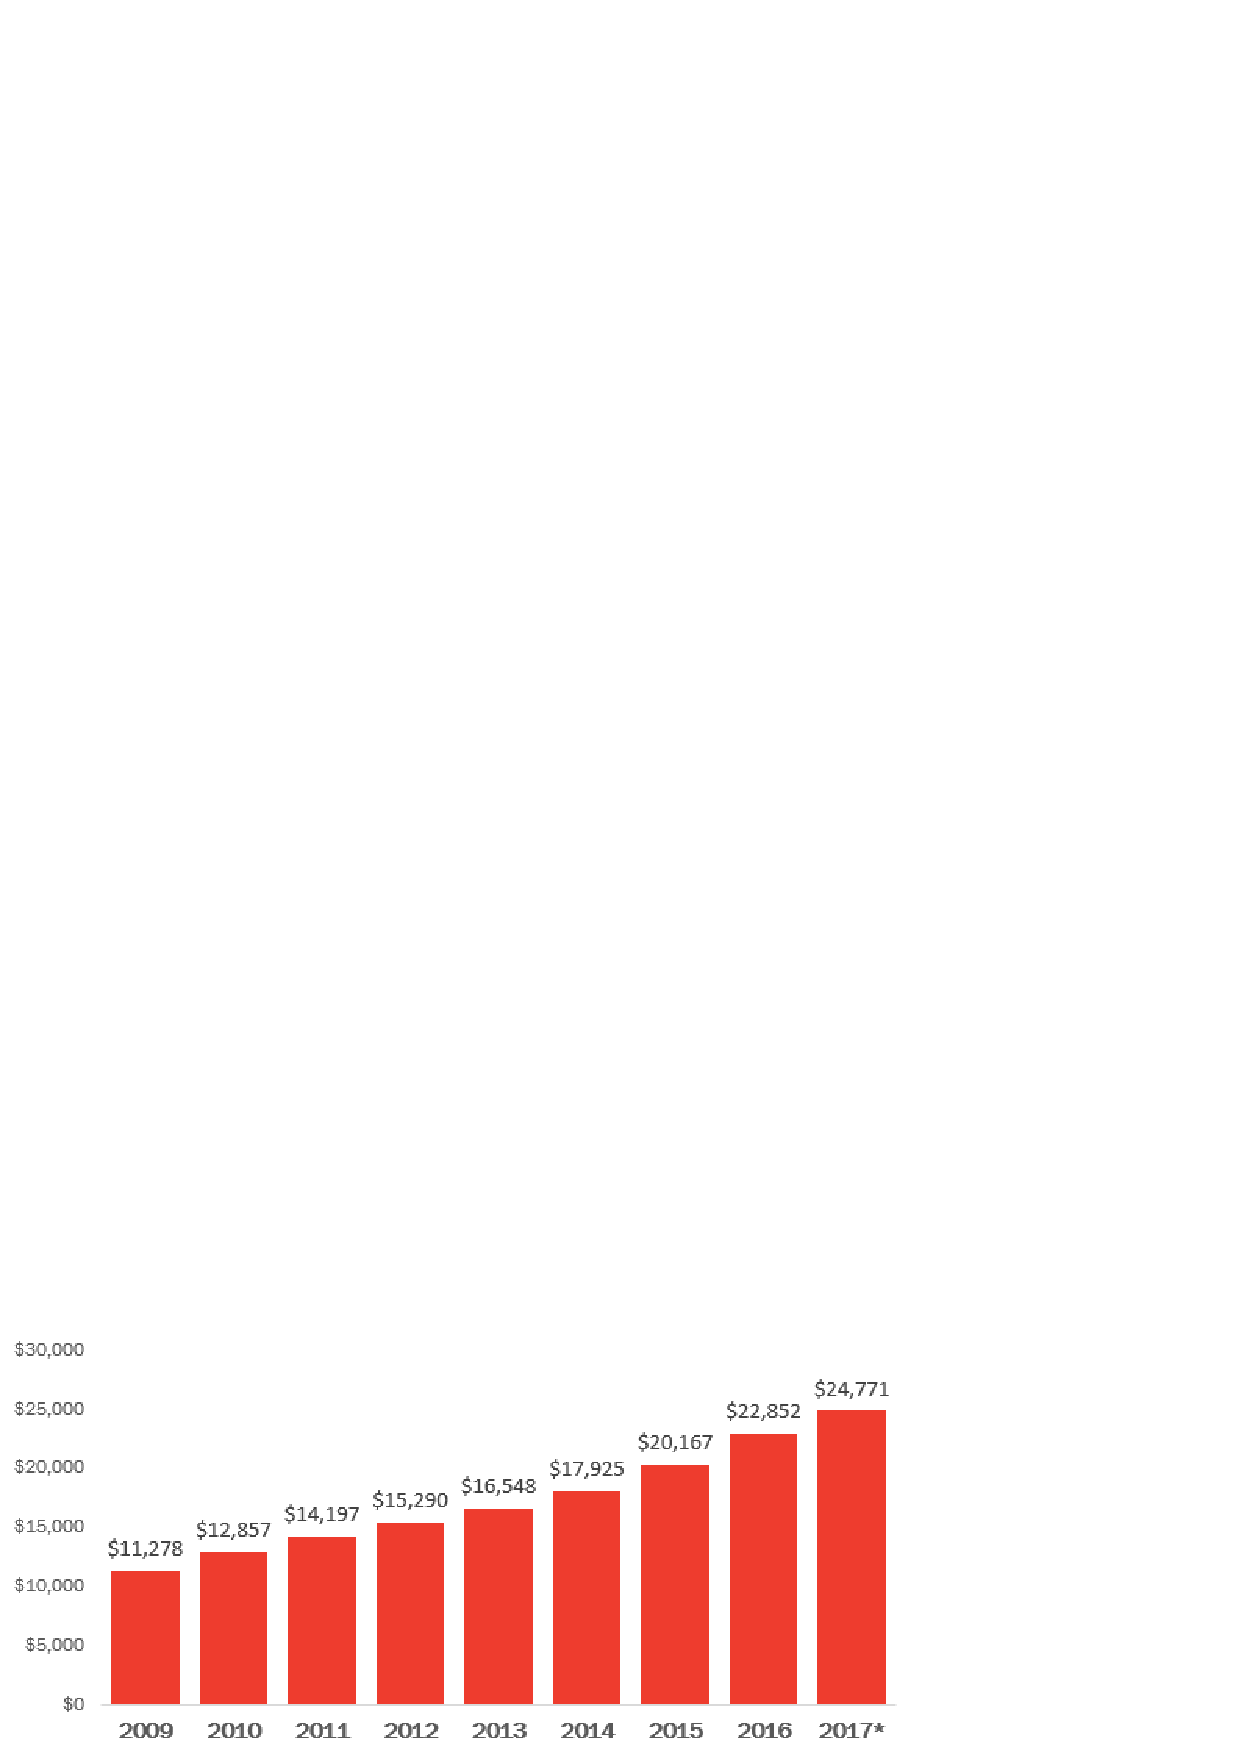
\includegraphics[width=0.5\textwidth]{03MarcoTeorico/imageR/merVidMex}
	\caption{Valor del mercado de videojuegos (Millones de pesos) elaborado por The Competitive Intelligence Unit (The CIU)[Imagen](2017). Recuperado de: http://the-ciu.net/nwsltr/152\_1Distro.html/}
	\label{fig:merVidMex}
\end{figure}

El teléfono móvil es el medio que ha mostrado mayor dinamismo en los videojuegos. Existen más de 90 millones de teléfonos inteligentes en uso dentro del país, lo que da acceso potencial a estas personas a miles de aplicaciones gratuitas y de paga existentes en el mercado. De esta manera, 66\% de los jugadores reportaron que utilizan su Smartphone, representando 39 millones de usuarios como se ve en la imagen \ref{fig:dispVid}. Y comprobamos el éxito potencial de los videojuegos en esta plataforma. Ahora veremos la frecuencia de juego que tienen las personas. 
\\[1pt] 	

\begin{figure}
	\centering
	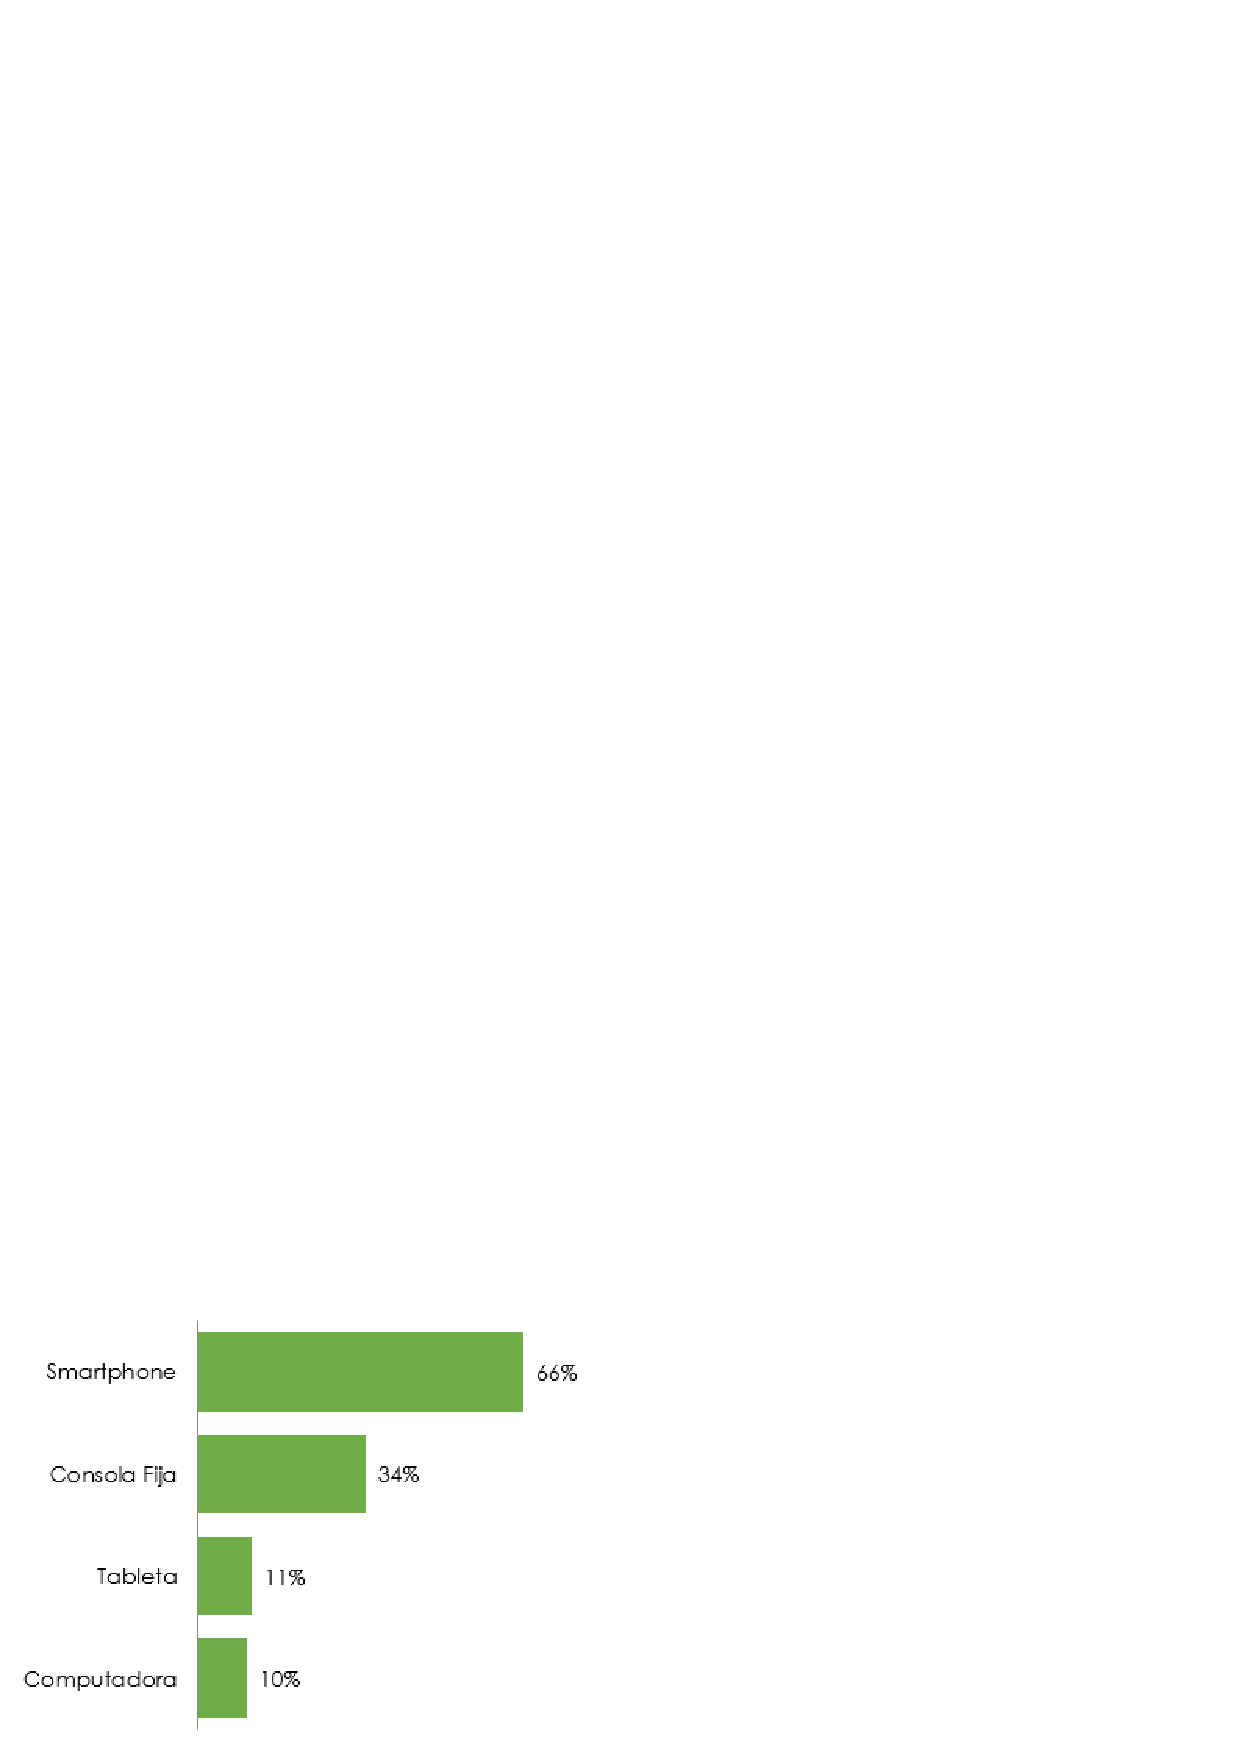
\includegraphics[width=0.5\textwidth]{03MarcoTeorico/imageR/dispVid}
	\caption{Grafica de dispositivos de acceso a videojuegos elaborado por The Competitive Intelligence Unit (The CIU)[Imagen](2017). Recuperado de: http://the-ciu.net/nwsltr/152\_1Distro.html/}
	\label{fig:dispVid}
\end{figure}

 El estudio revela que 63.7\% de los encuestados se asume como un usuario frecuente, que juega entre 1 y 3-4 veces a la semana; aunque de ese porcentaje el 40\% se asegura que juega entre una y dos veces por semana. Mientras que los ocasionales representan la parte menor con 5.4\%. De los llamado intensivos, por su parte, el 31.5\% juega diario o 5-6 veces a la semana como se ve en la imagen \ref{fig:frecJue}.
\\[1pt] 

\begin{figure}
	\centering
	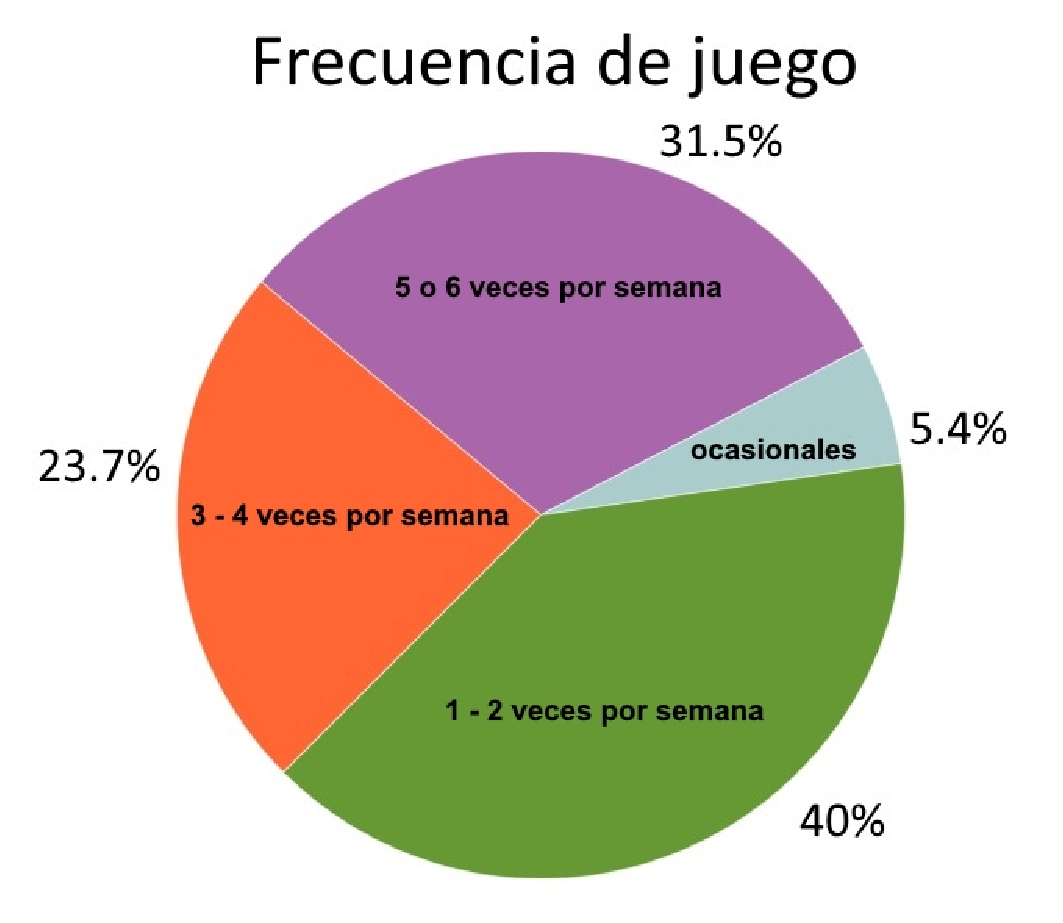
\includegraphics[width=0.5\textwidth]{03MarcoTeorico/imageR/frecJue}
	\caption{Grafica elaborada por encuesta de frecuencia de juego elaborado por The Competitive Intelligence Unit (The CIU)}
	\label{fig:frecJue}
\end{figure}

Así podemos concluir que en verdad México tiene mucha actividad dentro del consumo de videojuegos y convenientemente en una plataforma móvil.

\subsection{Industria en México}

La industria en México se refiere al desarrollo de videojuegos que existe dentro del país y no del consumo. La industria de producción de videojuegos en México se encuentra actualmente en una fase de desarrollo, debido a la persistente falta de oportunidades para desarrollarse en este tipo de actividad bajo un esquema corporativo o empresarial. Lo anterior se ve reflejado en la distribución del tipo de empleo de los desarrolladores nacionales, puesto que existe una alta proporción de empleados dedicados a la creación de videojuegos bajo un esquema independiente, son pocos casos los que llegan a consolidar su creación en una empresa con generación de empleos e ingresos en el largo plazo.
\\[1pt]

En México, la mayoría de empresas son micropymes, y no existe información abierta sobre su facturación o cuantas de ellas todavía no facturan. Muchas de estas pequeñas empresas recurren a soluciones como el crowndfounding mediante plataformas como Kickstarter para financiar su proyecto y buscan mentoring en las comunidades de desarrolladores cercanas\cite{vid05}. De acuerdo a estudios recientes, 40\% de los desarrolladores de videojuegos en México trabajan de modo independiente, mientras que únicamente 10\% de los desarrolladores han consolidado su propio negocio. Esto demuestra que una gran proporción de esta mano de obra se encuentra deslindada de grandes corporativos. En el caso de nuestro país como se ve en la imagen \ref{fig:desVj}, 6 de cada 10 desarrolladores dedican su actividad al desarrollo en smartphones y 32\% en tabletas, mientras que únicamente 26\% se especializan en el desarrollo de juegos en consolas fijas, respondiendo a una demanda de 40.7 millones de mexicanos que utilizan sus smartphones como principal dispositivo de juego \cite{vid04}.
\\[1pt]
\begin{figure}
	\centering
	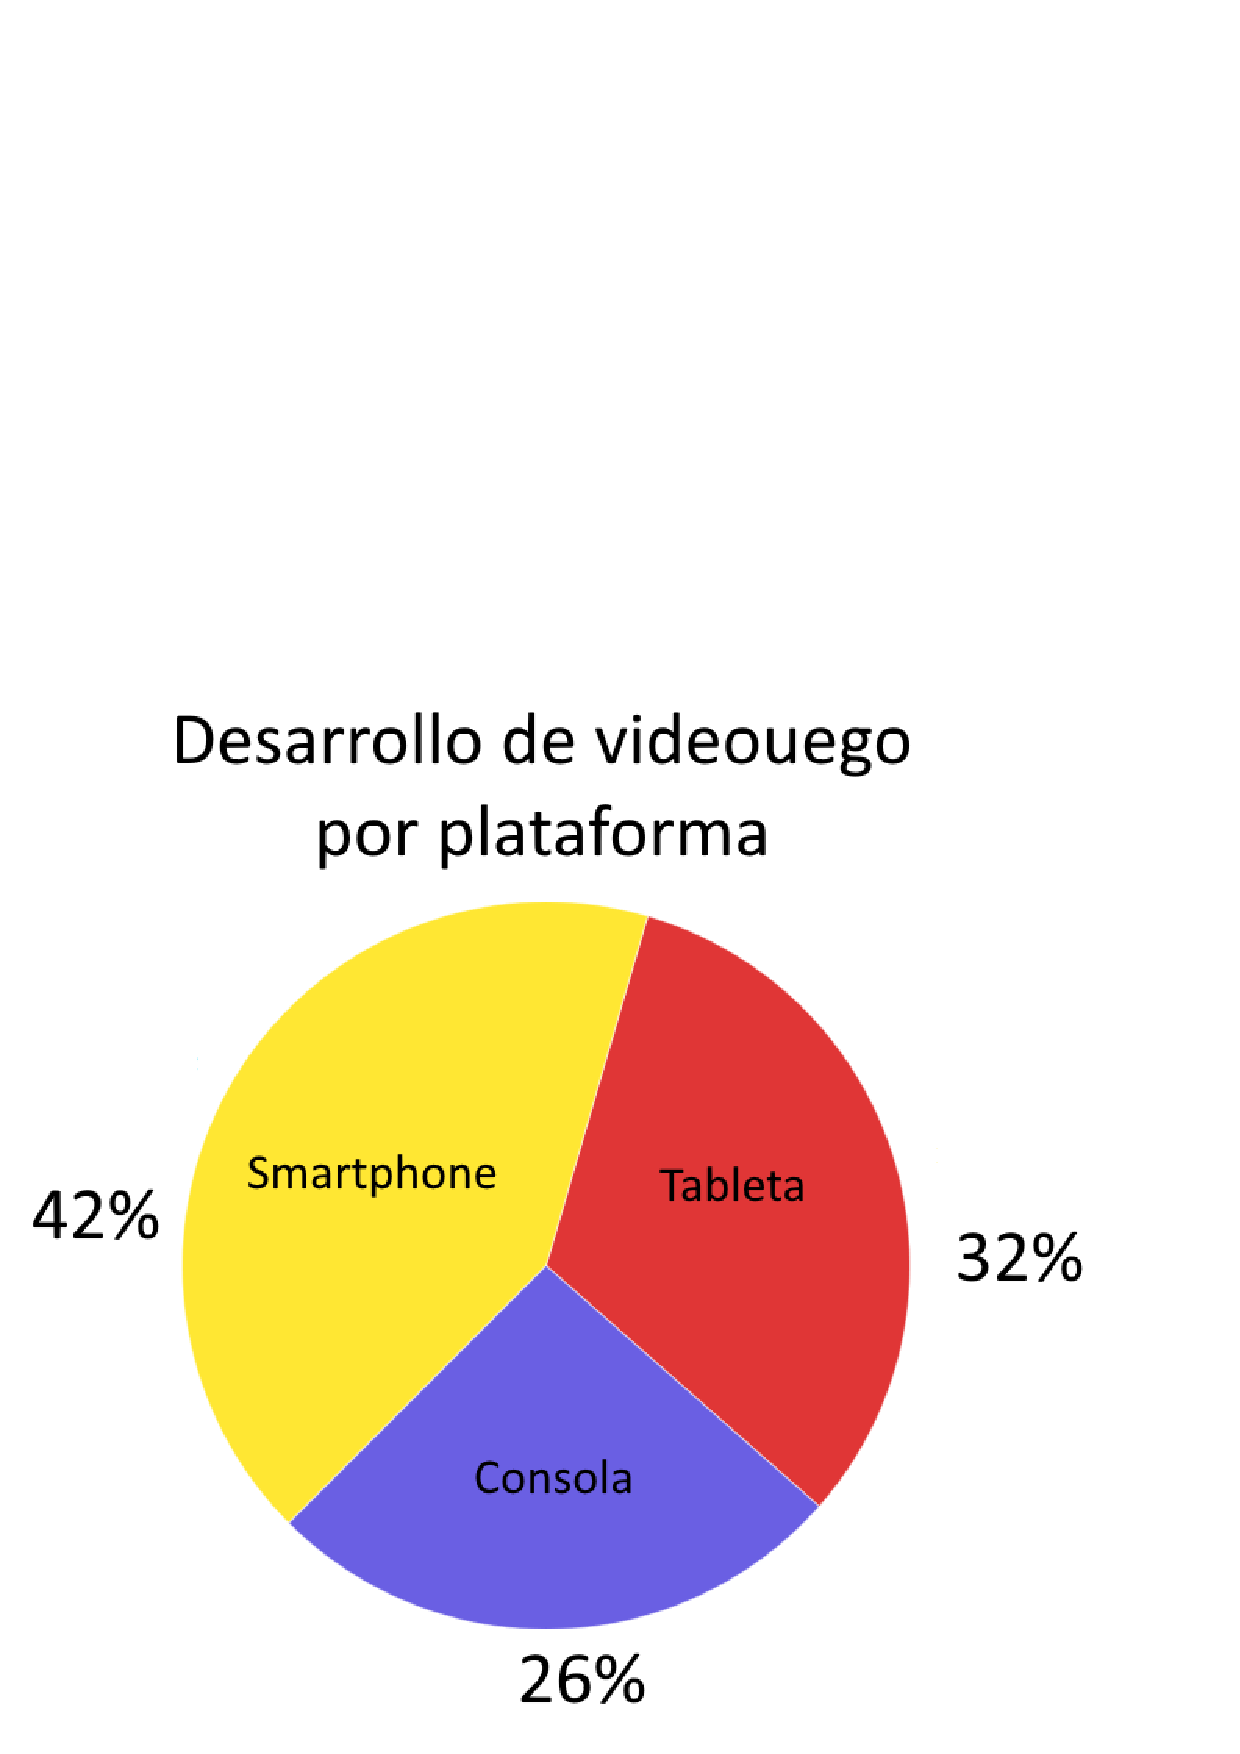
\includegraphics[width=0.3\textwidth]{03MarcoTeorico/imageR/desVj}
	\caption{Grafica de desarrollo de videojuego por plataforma en México realizada por encuesta de Competitive Intelligence Unit (The CIU).}
	\label{fig:desVj}
\end{figure}

Aquí una lista de estudios activos en México actualmente:
\begin{itemize}
	\item Larva Game Studios
	\item Kaxan Games
	\item Xibalba Studios
	\item Estudios Maquina Voladora
	\item Slang Studio
	\item Golden Pie Studio
	\item Kokonut Studio
	\item Phyne Games
	\item Playful Studios
	\item Squad Games
	\item Washa Washa
	\item Hollow Games
	\item HyperBeard Games
	
\end{itemize}
